%!TEX root = scivis_lbaakman_bvanloon.tex

\hypersetup{pageanchor=false}
\begin{titlepage}
    \centering
    \par\vspace{9cm}
    %{\scshape\LARGE University of Groningen \par}
          
            %\includegraphics[width=6cm]{img/logo.png} % also works with logo.pdf
    \par\vspace{3cm}
    {\huge\bfseries  Scientific Visualization \par}
    {\large\bfseries  An Interactive Application for Real-Time Simulation of Fluid Flow.\par}

    \vspace{1cm}\par
        
\includegraphics[width=0.42\textwidth, trim={35px 30px 430px 30px}, clip]{img/titlepage/zebra.png} \hspace{30px}
        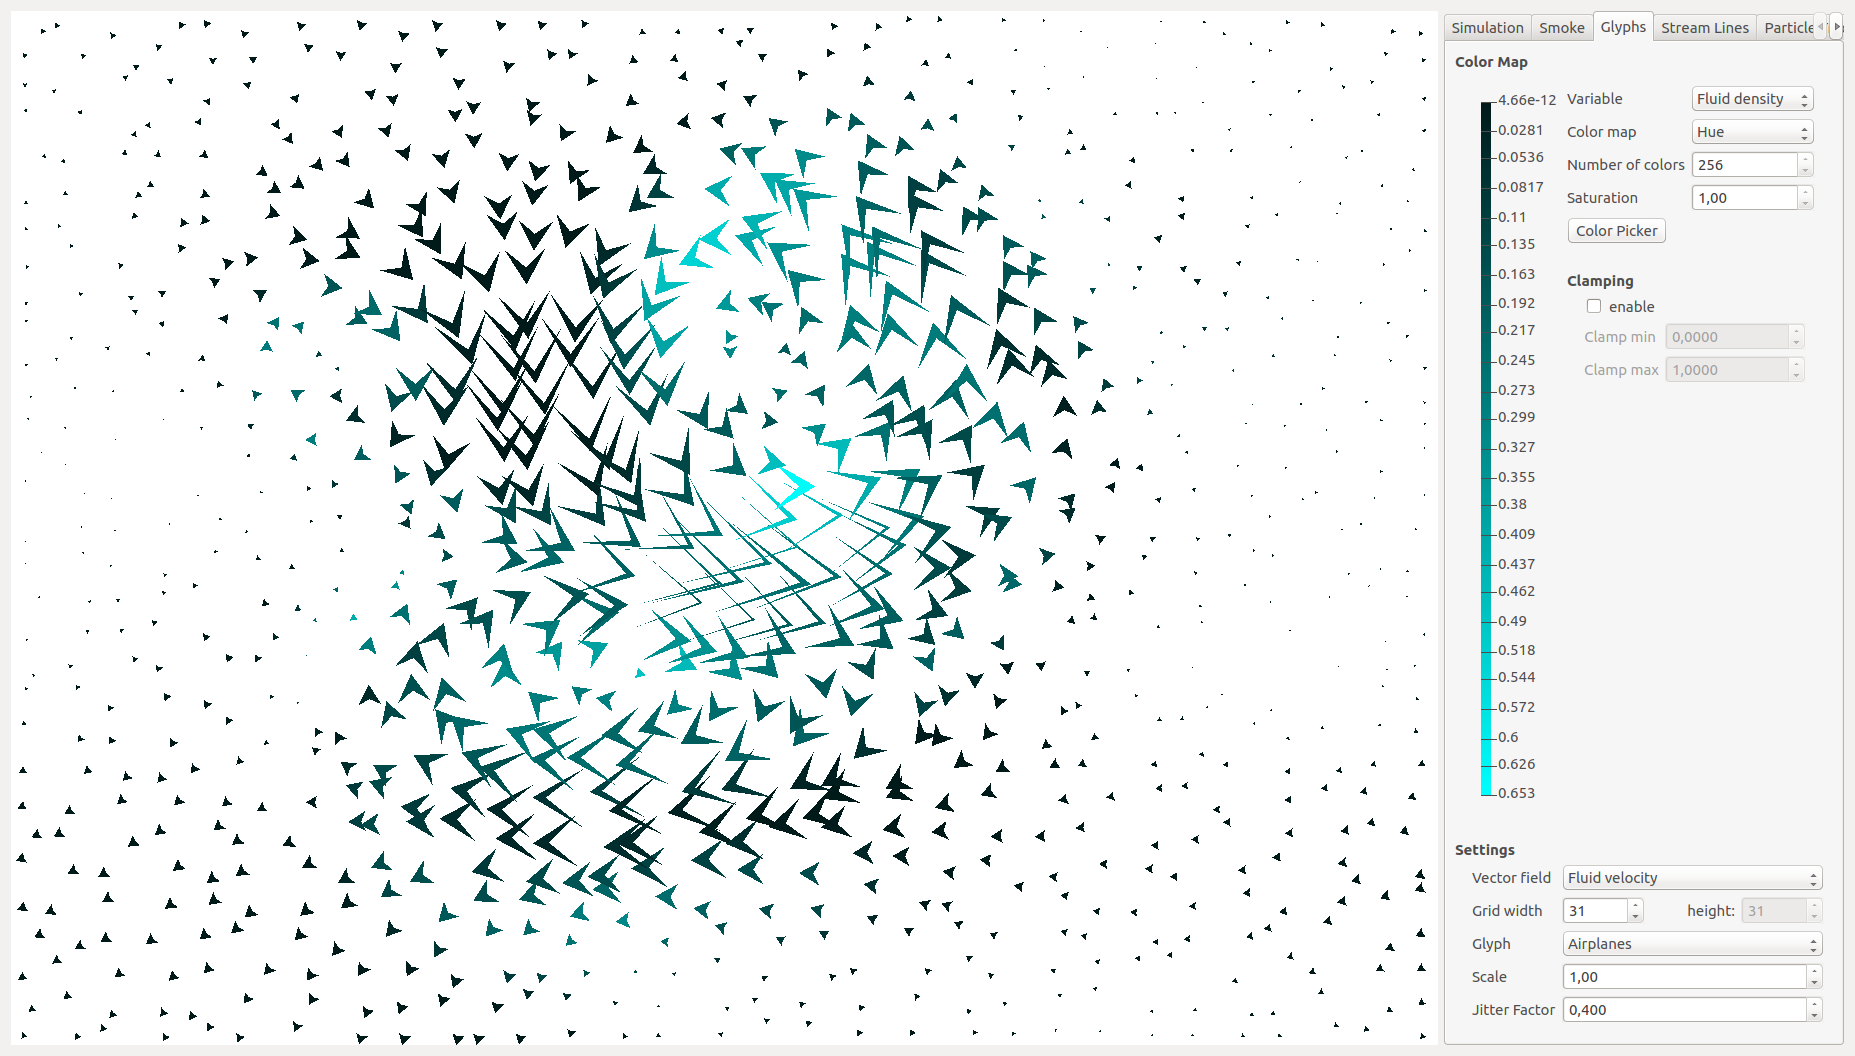
\includegraphics[width=0.42\textwidth, trim={35px 30px 430px 30px}, clip]{img/titlepage/glyphs2.png}

        \vspace{40px}
        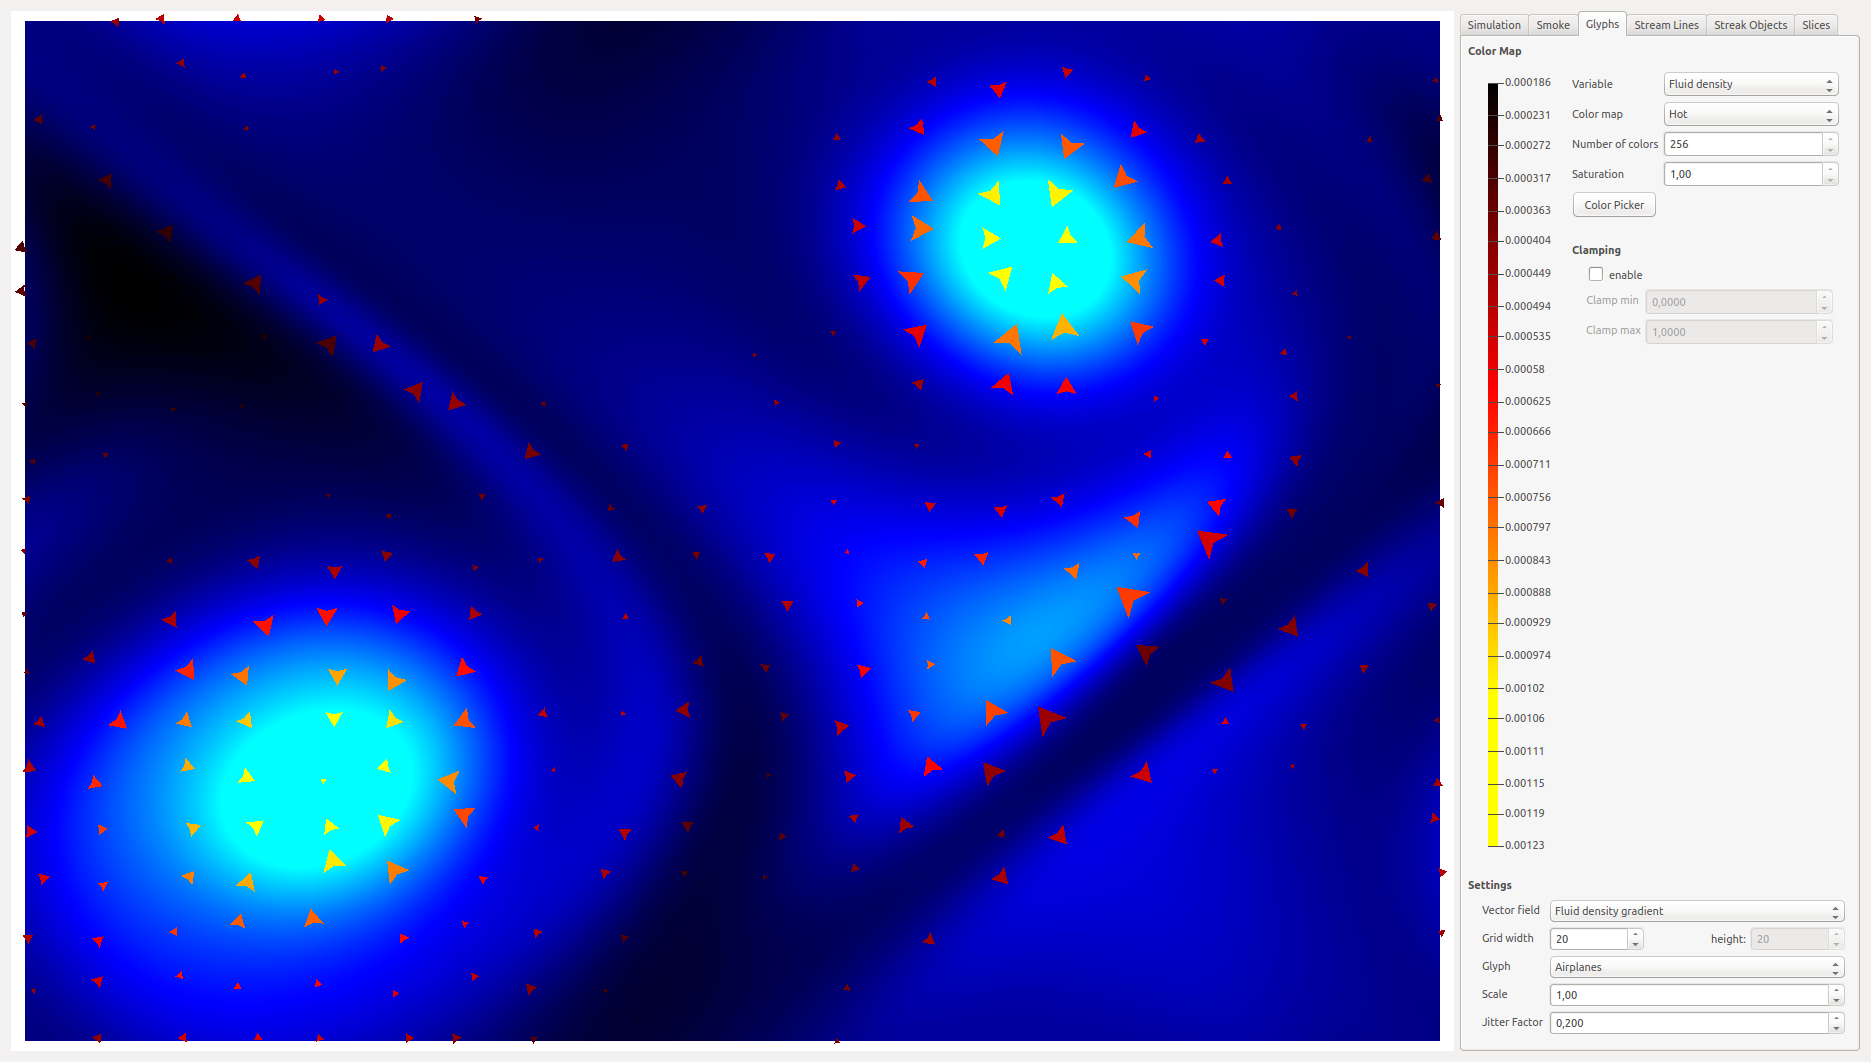
\includegraphics[width=0.42\textwidth, trim={35px 30px 430px 30px}, clip]{img/titlepage/gradient.png} \hspace{30px}
        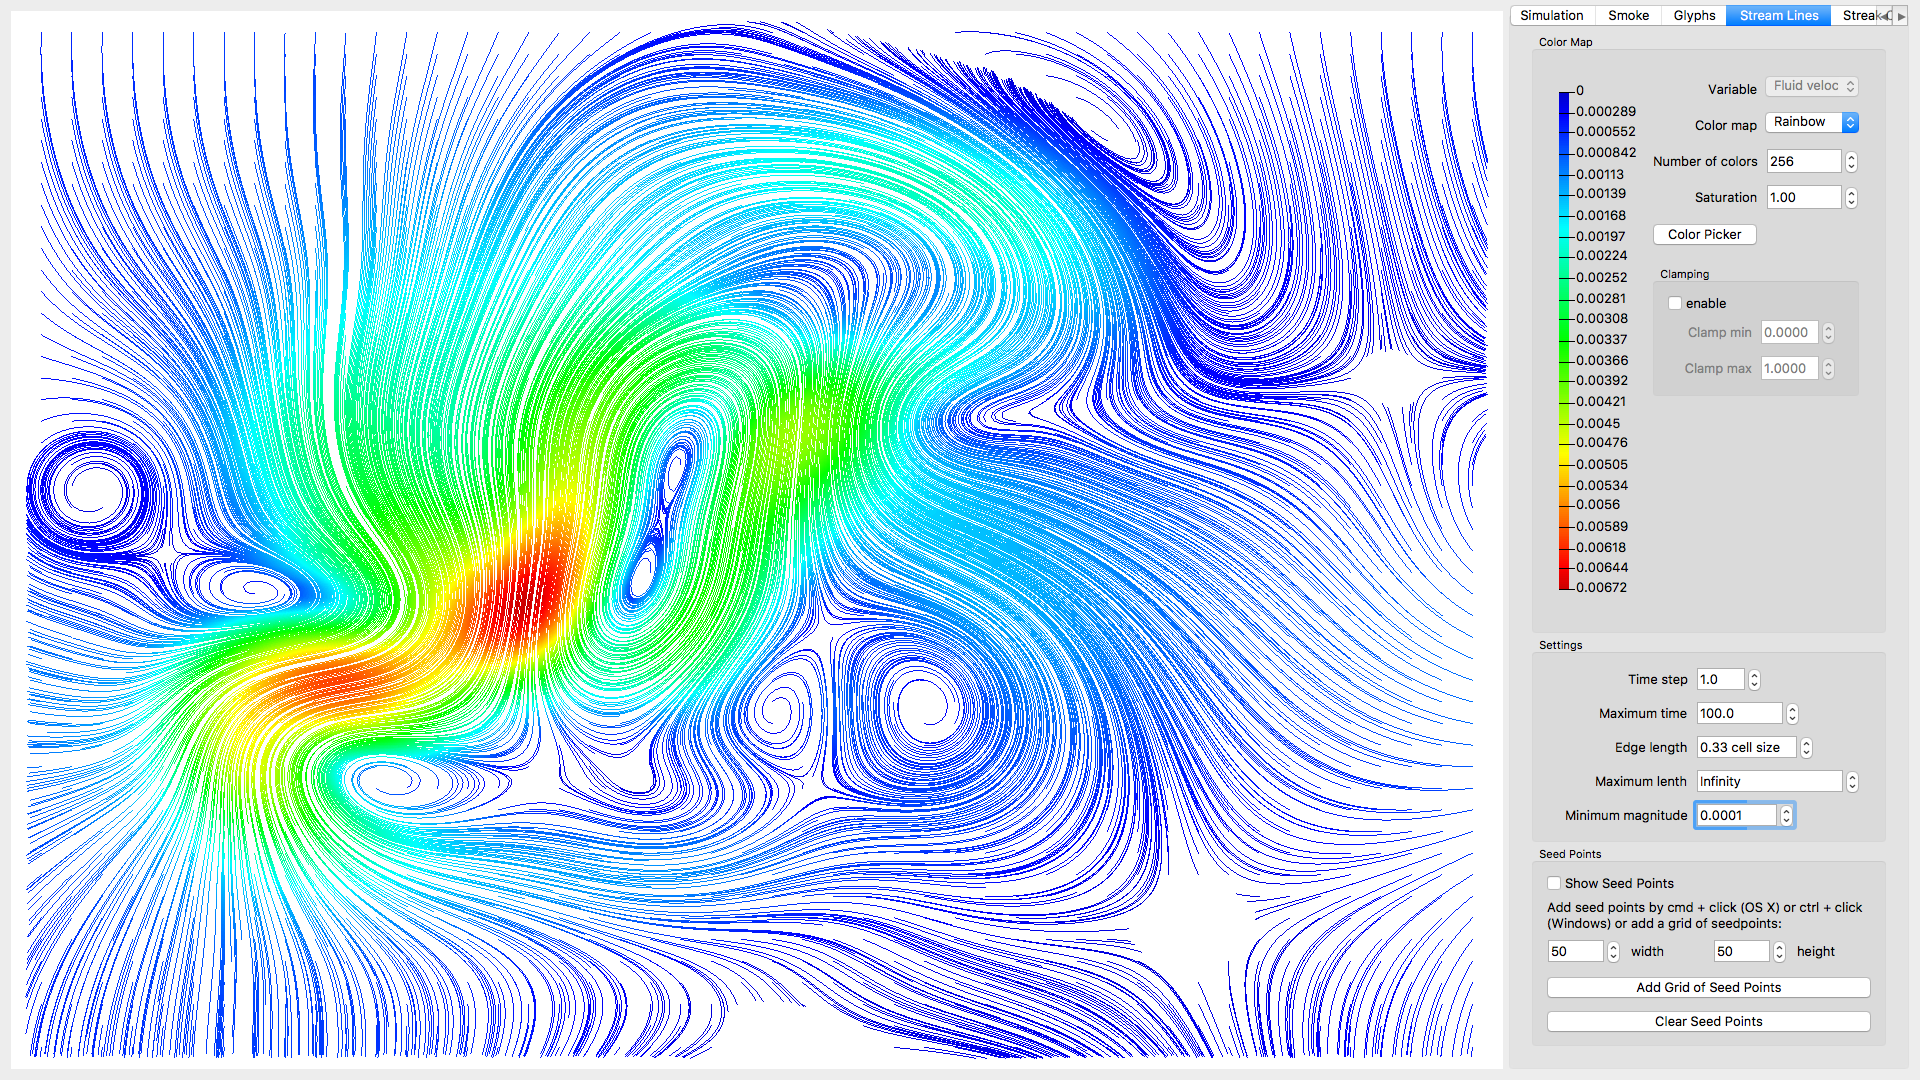
\includegraphics[width=0.42\textwidth, trim={35px 30px 430px 30px}, clip]{img/titlepage/streamlines.png}

        \vspace{40px}
        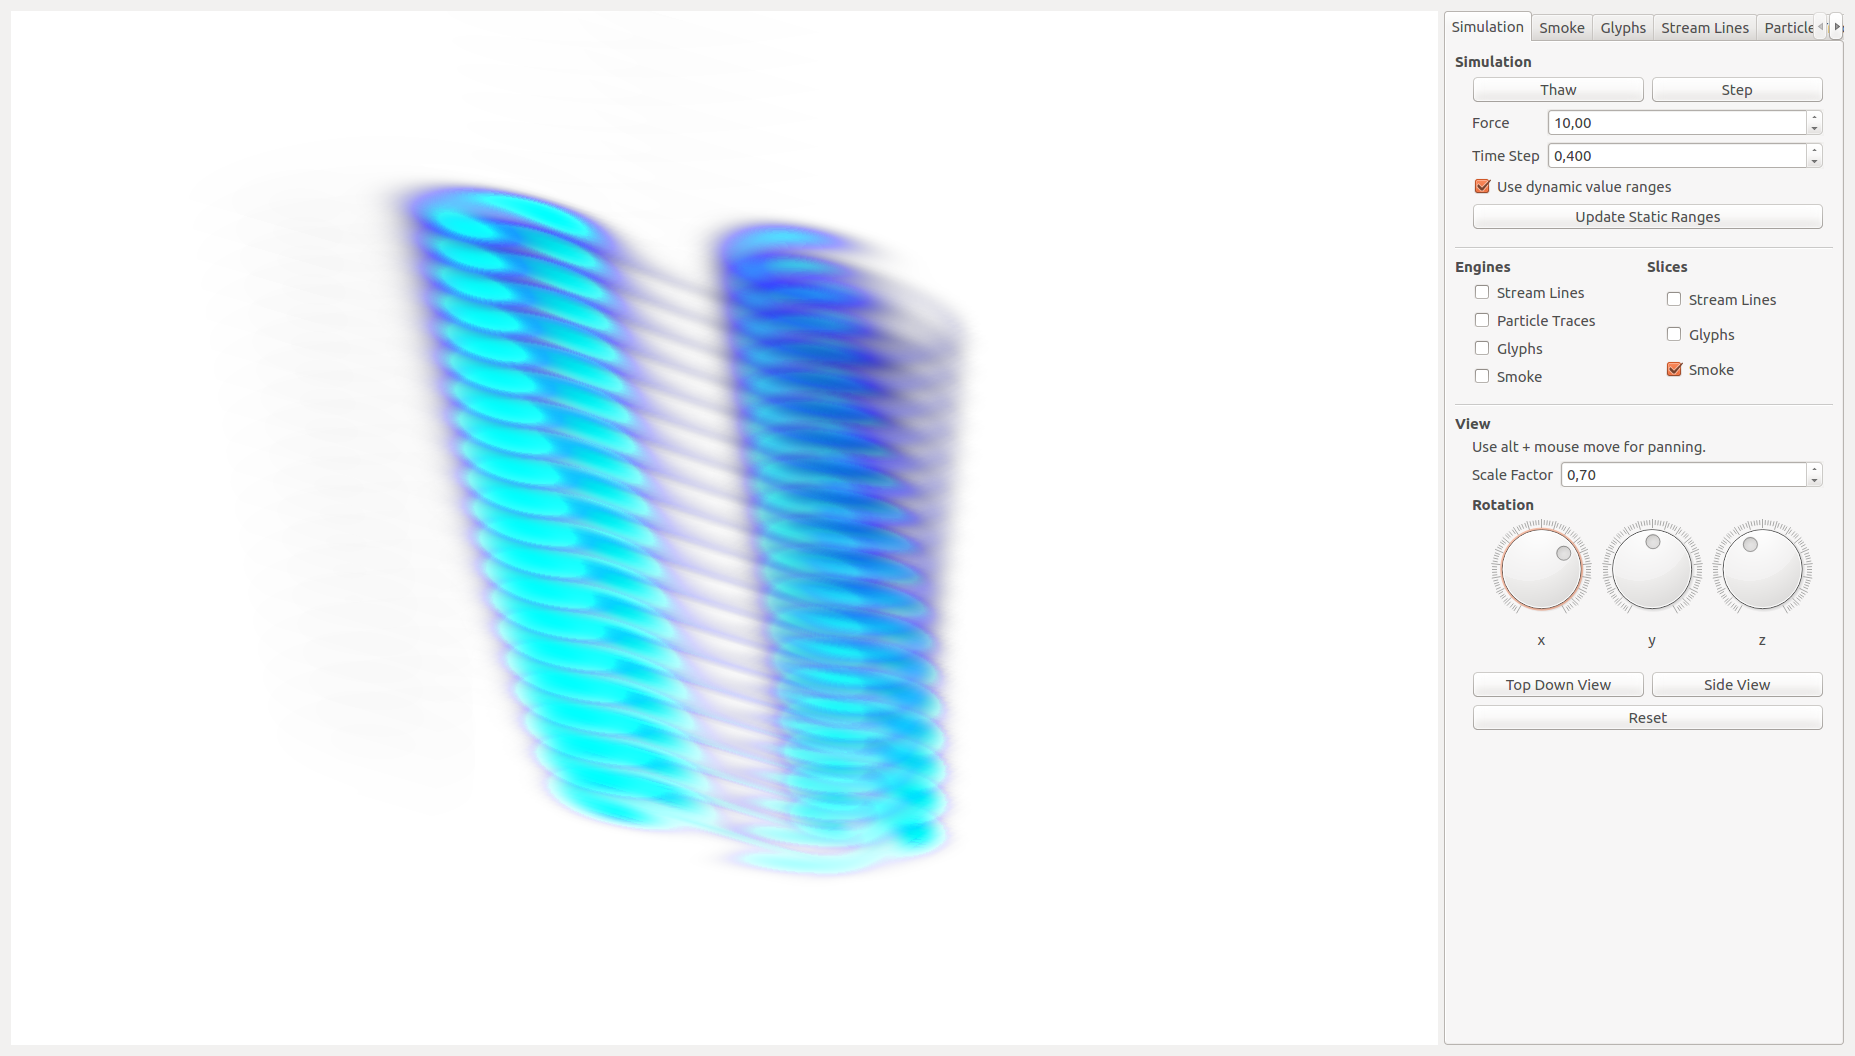
\includegraphics[width=0.42\textwidth, trim={35px 30px 430px 30px}, clip]{img/titlepage/slices2.png} \hspace{30px}
        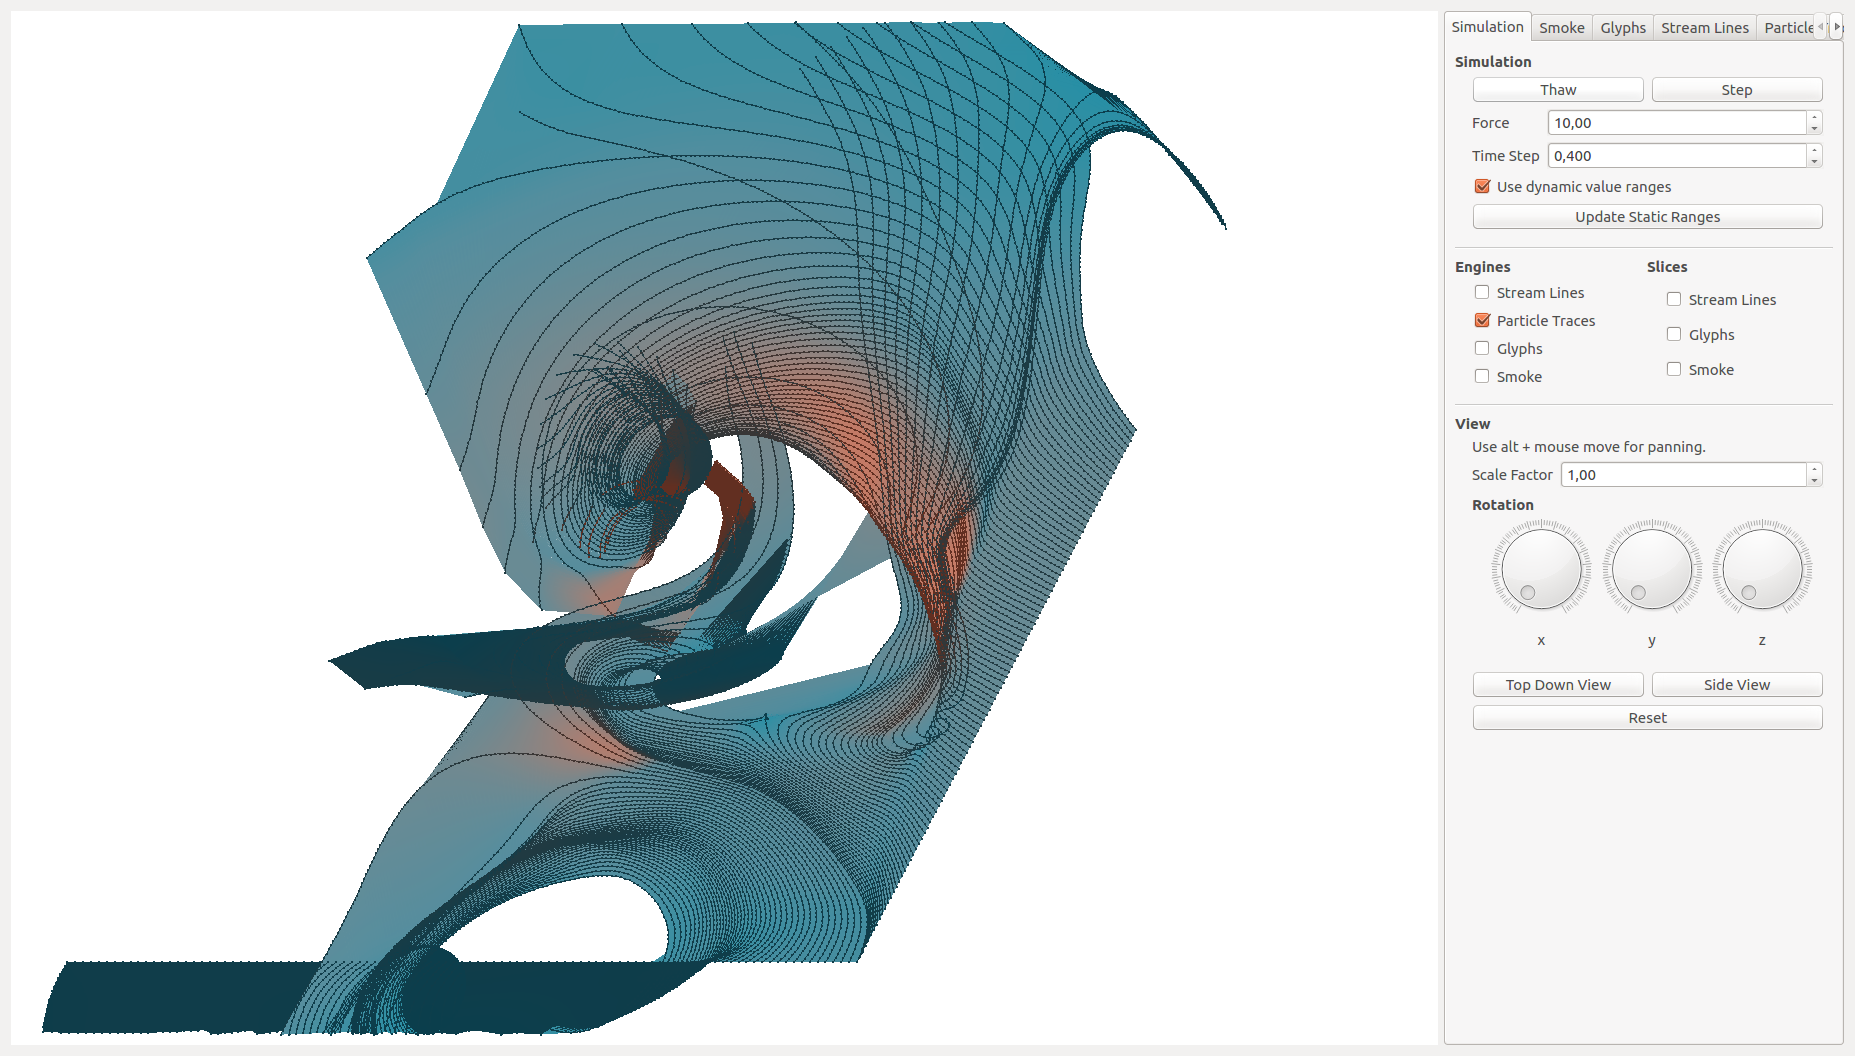
\includegraphics[width=0.42\textwidth, trim={35px 30px 430px 30px}, clip]{img/titlepage/particles.png}        
    \vspace{1cm}\par

    {\Large L.E.N. Baakman \textsc{s}1869140\par}
    {\Large S.J. van Loon \textsc{s}1795813\par}

    \vfill
% Bottom of the page
    {\large \today\par}
\end{titlepage}
\hypersetup{pageanchor=true}